%
% LaTeX template for prepartion of submissions to PLDI'16
%
% Requires temporary version of sigplanconf style file provided on
% PLDI'16 web site.
% 
%\documentclass[format=sigconf]{acmart}
%\documentclass[conference]{IEEEtran}
\documentclass[10pt,conference]{IEEEtran}

% \documentclass[pldi-cameraready]{sigplanconf-pldi16}

%
% the following standard packages may be helpful, but are not required
%
%\usepackage{SIunits}            % typset units correctly
%\usepackage{courier}            % standard fixed width font
\usepackage[scaled]{helvet} % see www.ctan.org/get/macros/latex/required/psnfss/psnfss2e.pdf
\usepackage{url}                  % format URLs
\usepackage{listings}          % format code
\usepackage{enumitem}      % adjust spacing in enums
\usepackage{graphicx}
\usepackage{amsmath}
\usepackage{mathtools}
%\usepackage{caption}
\usepackage{subcaption}
\usepackage{code}
%\usepackage[colorlinks=true,allcolors=blue,breaklinks,draft=false]{hyperref}   % hyperlinks, including DOIs and URLs in bibliography
% known bug: http://tex.stackexchange.com/questions/1522/pdfendlink-ended-up-in-different-nesting-level-than-pdfstartlink
%\newcommand{\doi}[1]{doi:~\href{http://dx.doi.org/#1}{\Hurl{#1}}}   % print a hyperlinked DOI


%\numberofauthors{2}

%\alignauthor
%Josie Holmes\\
%\alignauthor 
%Alex Groce\\
%      \affaddr{School of Informatics, Computing \& Cyber Systems}\\
%       \affaddr{Northern Arizona University
%}

%\setcopyright{rightsretained}
%\setcopyright{usgov}
%\setcopyright{usgovmixed}
%\setcopyright{cagov}
%\setcopyright{cagovmixed}


% DOI
%\acmDOI{10.475/123_4}

% ISBN
%\acmISBN{123-4567-24-567/08/06}

%Conference
%\acmConference[ISSTA'17]{International Symposium on Software Testing
 % and Analysis}{July 2017}{Santa Barbara, California, USA}
%\acmYear{2017}
%\copyrightyear{2017}

\newcommand{\comment}[1]{}

\begin{document}

\title{Does It Always Do That?  Practical Automatic Lightweight Nondeterminism
  and Flaky Test
  Detection and Debugging for Python Libraries}


\author{
\IEEEauthorblockN{Alex Groce}
\IEEEauthorblockA{School of Informatics, Computing \& Cyber Systems\\
Northern Arizona University\\
Email: agroce@gmail.com}
\and
\IEEEauthorblockN{Josie Holmes}
\IEEEauthorblockA{School of Informatics, Computing \& Cyber Systems\\
Northern Arizona University\\
Email: josie.holmes@nau.edu}}

%
% any author declaration will be ignored  when using 'pldi' option (for double blind review)
%

%\authorinfo{Person 1 \and Person 2}
%{\makebox{A Department} \\
%\makebox{A University}  \\
%\makebox{A Place, AS 12345}}
%{\{person1,person2\}@cs.auniv.edu}

%\begin{CCSXML}
%<ccs2012>
%<concept>
%<concept_id>10011007.10010940.10010992.10010998.10011001</concept_id>
%<concept_desc>Software and its engineering~Dynamic analysis</concept_desc>
%<concept_significance>500</concept_significance>
%</concept>
%<concept>
%<concept_id>10011007.10011074.10011099.10011102.10011103</concept_id>
%<concept_desc>Software and its engineering~Software testing and debugging</concept_desc>
%<concept_significance>500</concept_significance>
%</concept>
%</ccs2012>
%\end{CCSXML}

%\ccsdesc[500]{Software and its engineering~Dynamic analysis}
%\ccsdesc[500]{Software and its engineering~Software testing and debugging}

%\keywords{mutants, distance metrics, fault identification/localization}

\maketitle


\begin{abstract}
A critically important, but surprisingly neglected in the software testing literature, aspect of system reliability is system predictability.  Many software systems are implemented using mechanisms (unsafe languages, multiple threads, complex caching, stochastic algorithms, environmental dependencies) that can introduce behavioral nondeterminism.  Users of software systems, especially other software systems using library calls in a single-threaded context, often expect that systems will behave deterministically in the sense that they have predictable results from the same sequential series of operations.  Equally importantly, even when it does not impact correctness or user experience, nondeterminism must be understood and managed for effective (especially automated) testing.  Nondeterministic behavior that is not either controlled or accounted for can result in flaky tests as well as causing problems for test reduction, differential testing, and automated regression test generation.  We show that lightweight techniques, requiring (almost) no effort on the part of a developer, can be used to extend an existing test generation system to allow checking for problematic nondeterminism.  We introduce a set of lightweight nondeterminism properties, inspired by real faults, and tailor these notions to the practical, automatic, checking of Python library code.  In particular, we demonstrate that our proposed failure nondeterminism can improve mutation score by 6\% for a strong, full differential test harness for a widely used mock file system. 
\end{abstract}


\section{Introduction}

For ourselves, we might prefer to think (and act as if) we had free
will; however, we generally prefer our software systems to be as
constrained in their actions as possible:  in other words, we wish
them to be largely deterministic, from our perspective.

Determinism is particularly important for testing and debugging, where
being able to exactly reproduce system behavior is essential to
productivity \cite{Firesmith}.  If executing ``the same test'' can produce
significantly different behavior each time it is run, the consequences
can be unfortunate.  Developers using a test exhibiting nondeterminism
to debug a system
face a challenge in reasoning about causality, in that an event
observed may not even take place the next time the test is run; this
pernicious phenomenon has been sometimes referred to as the dreaded
``Heisenbug'' \cite{Heisenbug}, though the more accurate usage is
``Mandelbug'' \cite{GrottkeBugs,FaultTriggers}, since Heisenbugs, properly speaking, are bugs that disappear or
alter behavior under instrumentation (especially in debugging).
Automated test generation systems using test coverage results to drive
the search for interesting inputs may be mislead when a run executes
code only rarely.  And, most significantly, regression testing
effectiveness can be significantly reduced if tests fail only
intermittently and unpredictably, as a result of environmental
factors rather than bugs in changed code.  Such behavior is
unfortunately all too common:  Gao et
al. \cite{Gao:2015:MSU:2818754.2818764} observed coverage differences
of up to 184 lines of code for the same test, and false positive rates
as high as 96\%.  Nondeterminism is sometimes problematic for
developers, who will usually want to  assume that library code they
use is deterministic; it is frequently vexing in debugging efforts; it is often disastrous for large-scale highly
automated testing.


\subsection{What is Determinism?}

A system is deterministic if, given the system's complete state at a point in
time, it is possible, in principle, to predict its future behavior
perfectly.  We say ``in principle'' because in the real world,
prediction may be possible but hopelessly impractical.  We write
complex software systems in many cases because we cannot predict their
behavior (if we could perform the calculations in advance, ourselves,
we would just do so).  As a consequence, in software, rather than
defining determinism in terms of prediction, we usually therefore
simply say that a system is deterministic if, given the same state and
inputs, it always produces the same outputs.  

Technically, many ``nondeterministic'' systems are not
nondeterministic in a strong sense, at all.  Given the complete state
of the system (which includes the entire state of the underlying
hardware, the operating system, storage devices, etc.), ignoring
quantum effects, and treating outside interventions such as network
traffic, human activity at an input device, etc. properly as inputs,
most software \emph{is} completely predictable.  What we actually
mean, usually, is that, given a certain limited abstraction of state
and of inputs, observable behavior is repeatable.  This abstraction,
for most software, is not expected to include many elements outside of
the software system itself.

Because the
programmer's abstraction of the system ignores  such a large number of
details, very few tests are in fact ``deterministic'' in the sense
that they eliminate all changes in behavior between executions.  Running the same test
twice almost always results in differences, given a low enough level of
abstraction, since the system load,
cache contents, branch predictor history, etc. are almost never
controlled for; however, this kind of
nondeterminism is usually of no interest, unless the test involves
extremely precise timing constraints.  Rather, what matters is when
some kind of nondeterminism unexpectedly impacts computed values at a
higher level of abstraction; in general, if the operating system
itself is not buggy, low-level nondeterminism, by design, is invisible
except in fine-grained performance testing or real-time systems.
Unexpected nondeterminism usually arises when there is an element of higher-level
state or input that \emph{is} critical to the produced behavior, but
the programmer has not anticipated.  E.g.,  when it is believed that the
behavior of a thread scheduler will not matter, but a race condition
in the code means that it does matter, or when the order of items in
an iterator on a hash table is important, and the hash values used are
randomly salted.

\subsection{The High Cost of Unexpected Nondeterminism}

Unexpected nondeterminism is, unfortunately, usually only discovered
in a context that makes it very hard to debug.   The most common such
contexts are occasional rare failures of a system in deployment, and
regression tests that do not behave reliably (known as flaky tests).
Furthermore, unexpected nondeterminism makes it difficult to use
automated test generation to produce effective regression tests for a
system.  While developers may know how to produce reliably
deterministic unit tests, even in the presence of underlying
nondeterminism, automated test generation, without a large investment
in human time, usually does not have sufficient information to avoid
producing the occasional such test.  Moreover, where a human might
make an assertion about the final value produced during a unit test,
an automatically generated regression test is usually most easily produced by
simply asserting equality with all values produced during a reference
run, since the final step of a test
is likely to be somewhat arbitrary, generated in an effort to increase
code coverage, not establish some functional correctness property.
This may be one reason that automated testing is seldom used to
produce general regression tests.  While failure-inducing tests
produced automatically are often added to regression suites, the full
set of passing tests is, to our knowledge, only infrequently preserved
as part of a typical regression suite, perhaps because such tests are
likely to be \emph{flaky} without considerable human effort.

\subsubsection{Nondeterminism and Flaky Tests}

In order to help ensure that they are reliable and secure, complex
modern software systems usually include a large set of
\emph{regression tests}.  A regression test suite is a (usually large)
set of tests that can be run against a software system every time it
is modified, to ensure that the modification has not broken the system
in some way.  \emph{Flaky tests} \cite{miccoflaky} are regression
tests that fail in an intermittent, unreliable fashion, and thus
degrade the utility of regression testing.  The essence of a flaky
test is that, for the same snapshot of test code and code under test
(CUT), it sometimes fails and sometimes passes: the pass/fail result (disposition) of the
test is not a deterministic property of the test code, code under
test, and environment running the test.  This produces three serious
problems: first, a flaky test often wastes developer time and delays
software changes by forcing the investigation of code-under-test that
is not actually incorrect.  Second, failures in flaky tests (for that
reason) are often ignored, and therefore serious software faults may
be missed.  Finally, to mitigate these problems, flaky tests are often
run multiple times, wasting valuable computing resources and also
delaying acceptance of code changes.  An analogy may make the extent
of the problem in large-scale test automation clear:  a canary in a coal mine is of
little use if canaries frequently become ill for reasons unrelated to
the presence of toxic gases.  Mining may stop for no good reason, or
miners may learn to ignore the canary, leading to tragedy; a third,
more ``practical'' option is that miners may carry so many redundant
canaries into the coal mine that canary-care becomes a serious burden
on mining.

Flaky tests are, for us, simply a special case of general test
nondeterminism, where the nondeterminism of test values is sufficient
to cause the pass/fail result of the test to vary.  The definitions
and techniques proposed in this paper all apply to flaky tests, as a
special case of various kinds of \emph{horizontal} nondeterminism described below.

\subsection{Contributions:  Detecting and Debugging Nondeterminism}


This paper proposes (1) a number of formal definitions of types of
nondeterminism (\emph{horizontal} and \emph{vertical}) and (2) an implementation, based on these definitions, for detecting and debugging
nondeterminism in property-based testing.  The implementation is based
on an approach where (3) horizontal determinism is considered as a
kind of \emph{reflexive differential testing} and (4) vertical
determinism is specialized to the common case of \emph{failure determinsim}.
We further propose modifications to the widely used delta-debugging algorithm in order to better handle
nondeterminism as a test property

This enables a number of useful results:
 the automated production of
nondeterminism-free regression tests even for libraries with some
sources of nondeterminism, the documentation of
nondeterminism, and, most importantly, detection and effective debugging for
unexpected nondeterminism that is, itself, a bug.  We use a set
of case studies of real-world, widely-used, Python libraries to demonstrate the
utility of our ideas.  Failure determinism directly
produces a more than 5\% improvement in mutation score for an already highly
effective automated test generation tool for a file system, with no
additional specification or test design burden.
\section{Practical Lightweight Nondeterminism
  Detection and Debugging}



\subsection{Horizontal Determinism}

\subsubsection{Determinism and Reflexive Differential Testing}

Horizontal determinism can be best understood by thinking of
nondeterminism detection as an unusual kind of \emph{differential
  testing} \cite{Differential,ICSEDiff}.  In differential testing, a
system is compared against a reference in order to ensure that
it behaves equivalently, at some level of abstraction, to another
implementation of the same functionality.  Differential testing is
extremely powerful, in that any divergence of behavior, if divergence
is correctly defined, indicates a functional correctness fault in (at
least) one of the systems under test.  Being able to detect functional
correctness errors without the cost of constructing a formal
specification is extremely useful in automated test generation.  Differential testing is widely
used for systems software components such as compilers
\cite{Differential,csmith} and POSIX file systems \cite{CFV08,AMAI}, where multiple
implementations are common.  The major limitation of differential
testing, of course, is that multiple implementations of a system are
almost as rare as good correcteness specifications.

For the special case of detecting nondeterminism, however, \emph{a
  system can serve as its own reference implementation.}  

\subsubsection{Visible Value Determinism}

\subsubsection{Final State Determinism}

\subsubsection{Process-Level Determinism}

\subsection{Vertical Determinism}

Apple bugs.

\subsubsection{Failure Nondeterminism}

\subsection{Nondeterminism and Delta-Debugging}

Delta-debugging \cite{DD}\footnote{We use delta-debugging to stand for
  all test reduction algorithms, even those \cite{CReduce,tstl} that do not use the exact
  binary-search that distinguishes delta-debugging \emph{per se}; the
  differences are immaterial for our purposes.}  is a widely used method for reducing the
size of failing tests, making them easier to understand and debug.
Delta-debugging in the context of detecting nondeterminism has two
purposes.  One is simply the usual goal of reducing the size of a
test.  Identifying the cause of nondeterminism may be very easy in a
test consisting of ten library function calls (it is one of these ten
calls), but very difficult in a test consisting of a hundred library
function calls.  This is no different than the common use of
delta-debugging.  However, in nondeterminism detection,
delta-debugging can also be used to \emph{change the probability of
  nondeterministic behavior}.

In \emph{monotonic} cases, removing a part of a test cannot
increase the probability of a predicate holding.  This is fairly
common.  In these cases, when we use a reduction algorithm to reduce $t$
to $r$, $P(p(r) \leq P(p(t))$.  In \emph{non-monotonic} cases,
however, there is no such upper bound.  Removing a step in $t$ may
increase the probability that $t$ behaves nondeterministically.

The probabilistic predicate of interest for determinism is always of
the form:  {\bf the test will exhibit at least two different behaviors in $S$
runs, with probability $P$}.  This predicate may be monotonic or
non-monotonic, depending on the causes of the nondeterminism detected.

The only absolutely necessary changes required to use standard
delta-debugging implementations in nondeterminism detection
are simply removal of some ``sanity checks'' in the code:  many
implementations (including the Python code provided by Zeller) assert
that the predicate holds on the original test.  In probabilistic
settings, this may not be true, and we may even be trying to find a
subset where a predicate that is very far from holding on the original test
holds (in a non-monotonic case where we aim to increase the probability
of nondeterminism).

\subsubsection{``Publication Bias'' in Delta-Debugging}

However, simply using delta-debugging off the shelf with a predicate
like $P(fail) > 0.3 \wedge P(fail) < 1.0$, to force a test to be flaky, and force it to fail
sufficiently often to be used in debugging, will often produce
surprising and unfortunate results.  In many cases,
delta-debugging will indeed reduce the large test to a small subset.
And, in a technical sense, delta-debugging will work:  it will never
convert a nondeterministic test to a completely deterministic test,
because the reduced test that delta-debugging returns is always one
where the predicate of interest has been seen to evaluate to true.
However, if you run the resulting test, it will, in many cases, have a
$P(fail)$ that is much, much smaller than
0.3, perhaps as low as 0.01.  Why?

The problem is analogous to the problem of publication bias in
scientific fields \cite{ahmed2012assessment}.  A predicate like
$P(fail) > 0.3 \wedge P(fail) < 1.0$ cannot be evaluated by
determining the true probability of failure; rather, the test must be
run some concrete number of times, and the number of failures counted.
However, even if the number of samples $N$ is large, there is some
probability (based on the sample size) of a result that diverges
significantly from the actual probability of failure.  If the
predicate were run only once, and the number of samples reasonably
large, this would not matter.  However, by their nature,
delta-debugging and other test reduction algorithms, explore a search
space that often contains hundreds or even thousands or millions of
candidate tests.  The predicate is evaluated on each of these, and so
even with large $N$, it is extremely likely that some evaluation will
produce a very poor estimate of $P(fail)$.  If such an evaluation
causes the predicate to appear to hold for a test, delta-debugging is
``stuck'' with the error, because (to our knowledge) no test reduction
algorithms allow backtracking.  After such a mistake, finding further
reductions will become harder, but may still be possible due to the
same source of errors:  the number of experiments run is far larger
than the probability of an incorrect result.

It is the combination of
a one-way bias on faulty evaluations (the consequences of a false
positive for the predicate are much greater than for a false negative)
and the huge number of experiments relative to error rate, that
produces bad results, akin to the magnification of effect sizes
in science due to publication bias.  The bias in delta-debugging tends
towards producing a reduced test where probabilities are much smaller
than demanded by a predicate, due to the pressure on delta-debugging
to produce shorter tests.  Shorter tests have smaller probabilities,
on average, due to two factors:  first, timing-induced nondeterminism
has a much smaller temporal space to operate in, and second, if some
test operation introduces a small probability of nondeterminism, and
only many repetitions of that operation make the probability large,
small tests obviously on average have fewer instances of the
problematic operation.

In scientific literature, the most frequently proposed solution is the
use of replications:  repeated runs of ``successful'' experiments to
minimize the probability that a result is a fluke due to publication
bias.  One way to produce this effect would be to allow
delta-debugging to backtrack if the probabilties observed in predicate
evaluations suddely exhibit a strong discontinuity, a kind of ``paper
retraction'' based on near-replications.  However, this requires
modifying the delta-debugging implementations, which is difficult and
sometimes not really feasible (e.g., few users of AFL-fuzz \cite{aflfuzz} will wish
to change its C code for test reduction).  Ideally, the solution
should be implementable simply by modifying the predictate that is
evaluated.  

A costly but effective solution is to make $N$ large in comparison to
the number of expected predicate evaluations performed during
delta-debugging.  If the error rate is low enough, the problem
disappears.  However, given the large number of evaluations performed,
this will tend to make delta-debugging extremely slow.  We propose
using a dynamic sampling approach, where $N$ is small, but if the
predicate evaluates to true, $M$ repeated true evaluations
(``replications'') are
required before the predicate returns ``true'' to the delta-debugging
algorithm.  A set of $M$ repeated false positives with
$\frac{N}{M}$ samples each is much less likely than a false positive
with $N$ samples; so long as we accept the resulting bias in favor of
false negatives, we can therefore produce a reduced test with a
desired $P(fail)$ much more cheaply:  the use of replications not only
means we only pay the full sampling price on rare occasions, but a
desired accuracy for $P$ can be obtained with a much smaller value $M
\times N$ than a non-dynamically-sampled $N$.  For example, if we the predicate
is $P(fail) \geq 0.5$, and the true probability for a candidate test
is 0.25, using $N=8$ will give a false positive rate of over 10\%.
Using 4 replications on just 2 samples ($M=4;N=2$) yields a false
positive rate of about 3.7\%, yet requires almost 60\% fewer
executions of the test\footnote{The probability calculations for such comparisons
  are relatively simple, but in real testing are
  usually not very useful, since the true
  probabilitiy distributions of test behaviors vary widely and
  dynamically during the
  delta-debugging process, making exact calculation unwieldy, even if
  the changing probabilities were known; exact results would be based on fictional
  probabilities, so gathering experimental data during a trial
  delta-debugging run and tuning $N$ and $M$ to yield desired
  results is  more effective.}.

Tuning $M$, any degree of confidence can be achieved, with
the basic tradeoff being between finding a test with the desired
probabilities, and the speed and effectiveness of delta-debugging.
Because increasing $M$ makes false negatives more likely, larger $M$
will usually result in less-than-optimal reduction of the original
test.
\section{Implementation}

\subsection{Sources of Nondeterminism in Practice}

\subsubsection{Process-Based Nondeterminism}

Address Space Layout Randomization (ASLR) \cite{ASLR} 

\subsection{Implementing Nondeterminism Detection}

We implemented our approach in the TSTL \cite{NFM15} system.

Because TSTL supports differential testing \cite{tstlsttt}, horizontal
nondeterminism detection can technically be implemented simply by
declaring a system to be its own reference, using TSTL's notation for
differential testing.  However, such an approach requires some effort
on the part of the user to control which values are checked for
equivalence, and does not easily support injecting timing differences,
or using a new process, in checking the behavior.



Because TSTL has an interface to afl \cite{aflfuzz}, we can even use
afl's sophisticated heuristics to perform very thorough, week-long
checks for nondeterminism, using strategies built to find subtle
security vulnerabilities in C programs.
\section{Experimental Evaluation}

In order to evaluate our approach and implementation, we applied
nondeterminism detection to real Python code, including some widely
used libraries (according to GitHub, {\tt pyfakefs} is used by at least
338 other projects, and {\tt redis-py} is used by at least 50,000).  The primary
points we wanted to explore were {\bf RQ1:} whether our approach was able to reliably detect actual
nondeterminism, {\bf RQ2:} whether the overhead of nondeterminism
detection for real systems was acceptable, and {\bf RQ3:} whether the performance of
delta-debugging in this setting was acceptable, in terms of both time
and results (amount of reduction).  We chose two of
the subjects, {\tt redis-py} and {\tt pyfakefs}, based on the fact that they were previously-existing large
TSTL harnesses, and serve to show how easily our
approach can be integrated into an existing test
generation effort.  The other two subjects were chosen, and new harnesses
written, specifically to demonstrate specific, important sources of
nondeterminism in Python code: concurrency and hash salting.
\begin{comment}In
addition to our core research questions ({\bf RQ1-RQ3}) shared by all subjects, we
report on aspects of using the TSTL nondeterminism tools
specific to each subject.
\end{comment}
Table \ref{tab:overviewexp} shows a summary of our experimental
results.  In all cases, our approach was able to detect interesting
nondeterminism (in fact, all nondeterminism of which we are aware).  The overhead imposed by nondeterminism
checks varied,, but in the worst case did not double the
average cost of each action (the expected overhead, since we
essentially execute each test twice), and thus never halved the amount of
testing.  Test reduction always reduced the size of
generated tests by 85\% or more, in less than 15 minutes, thus showing that reduction
has a large payoff at an acceptable price.  Values are, unless otherwise noted, the mean of 30 runs.

\begin{table}
  \centering
  {\scriptsize
\begin{tabular}{l|l|r|r|l}
& \multicolumn{1}{c}{\bf RQ1} & \multicolumn{1}{|c|}{\bf RQ2} &
                                                              \multicolumn{2}{c}{\bf RQ3}\\
  \hline
Subject & Detection & Overhead & Reduction \%
                                                        & Reduction time\\
\hline
Parallel Sort & Yes (see below) & $\sim$40\% & $\sim$85\% & $\sim$2 minutes\\
{\tt redis-py} & Yes (see below) & $\sim$20\% & $\sim$95\% & $\sim$10 minutes\\
{\tt datarray} & Yes (see below) & $\sim$93\% & $\sim$90\% & $\sim$92
  seconds\\
{\tt pyfakefs} & Yes (see below) & $\sim$8\% & $\sim$99\% & $\sim$1 second  \\
\end{tabular}
}
\caption{Overview of experimental results}
\label{tab:overviewexp}
\end{table}

\subsection{Parallel Sorting}

Our first subject is an implementation of a parallel merge
sort ({\url{https://gist.github.com/stephenmcd/39ded69946155930c347}). When a sorting
algorithm is implemented using concurrency, a key question to ask is
whether the ordering of (equal under comparison) elements is
consistent.  TSTL can be used to show that a parallel sort implementation provides
a consistent, deterministic ordering.
\begin{comment}
This is related to the question of whether a sort is stable,
but imposes a less strict requirement; a concurrent sort
might not be stable, but might still produce the same (non-stable)
ordering from the same provided sequence, every time.  While a parallel
implementation of an algorithm will likely have internal
nondeterminism, it is often expected to
behave deterministically, from the point of view of a caller.

This experimental subject serves two purposes:  first, to show that the
nondeterminism detection features of TSTL can be used to, with
acceptable overhead, show that a parallel sort implementation provides
a consistent, deterministic ordering, and second to show that the
mechanism can also detect the nondeterminism in a parallel sort that
does exhibit nondeterministic behavior.
\end{comment}
For contrast, we also 
implemented a very simple swap-based parallel sorting algorithm that
repeatedly has multiple threads scan through a sequence and swap
out-of-order neighbors, until the sequence is sorted (a kind of
parallel bubble-sort).

\begin{comment}
\begin{figure}
{\scriptsize
\begin{code}
@import mergesort
@import swapsort

pool: <val> 10
pool: <data> 10
pool: <sorted> 10

<val> := <[-10..10]>

<data> := []
<data>.append((<val>,<val>))
len(<data,2>) < len(<data,1>) -> <data>.extend(<data>)

<sorted> := mergesort.merge\_sort\_parallel(<data>)
<sorted> := swapsort.swap\_sort\_parallel(<data>)
<sorted>

property: swapsort.is\_sorted(<sorted>)
\end{code}
}
\caption {Complete TSTL harness for checking two parallel sorting
  algorithms for nondeterminism.}
\label{fig:parallelcode}
\end{figure}

Figure \ref{fig:parallelcode} shows the complete TSTL harness for
checking the parallel sorts.
\end{comment}

Our TSTL harness for parallel sorting produces sequences of
integer pairs, where only the first integer is used in the comparison
operator of the sorting algorithms, and checks that the results of
are sorted..
Both sorting algorithms always produce sorted output.  The
horizontal determinism detector, however, always generates a 
test case showing the {\tt swapsort} behaving nondeterministically in
less than 3 seconds, thus
answering yes to {\bf  RQ1}.  If we comment out the call to {\tt
  swap\_sort\_parallel} and only check the parallel merge sort, TSTL
finds no nondeterminism.  This results in a slowdown of approximately
40\% ({\bf RQ2}).

Reducing a lengthy test showing nondeterminism of the swapsort usually takes less than two
minutes (out of 10 trials, only one took four minutes).  The resulting test will be usually be very compact, e.g.
reducing the original test from 56 to 8 steps.

\begin{comment}
{\scriptsize
\begin{code}
data0 = []    
val0 = 3      
val1 = -9    
data0.append((val0,val1)) 
val2 = -1                         
data0.append((val1,val2))
data0.append((val1,val1))  
sorted0 = swapsort.swap\_sort\_parallel(data0)      
\end{code}
}
\end{comment}
%For this simple example, more sophisticated reduction strategies
%are not needed; we only want to see the code behaving
%nondeterministically, and do not care about preserving a higher probability of nondeterminism.

\subsection {The {\tt redis-py} Library}


\begin{figure}
\centering 
\begin{subfigure}{0.3\columnwidth}
\centering
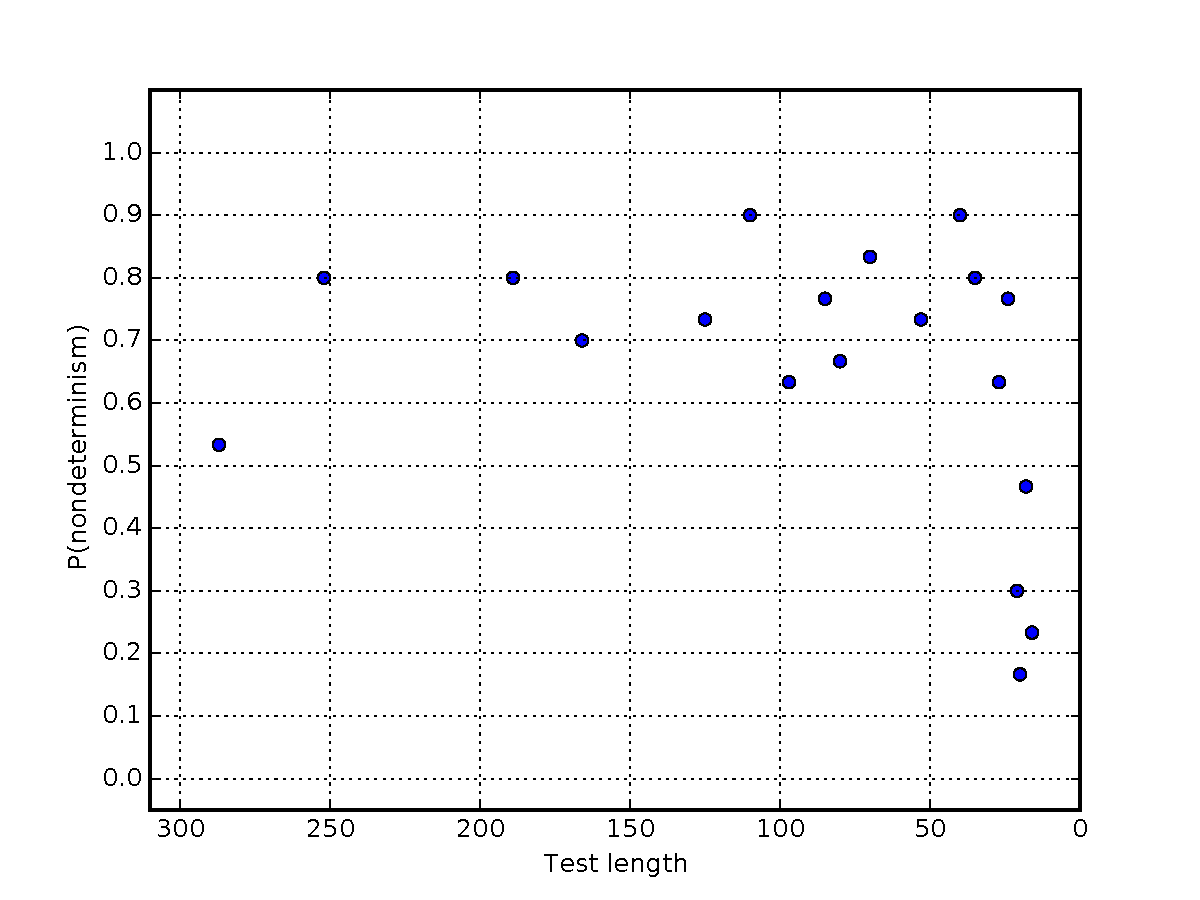
\includegraphics[width=\columnwidth]{redisddmin}
\caption{No modification}
\label{fig:r1}
\end{subfigure}
\begin{subfigure}{0.3\columnwidth}
\centering
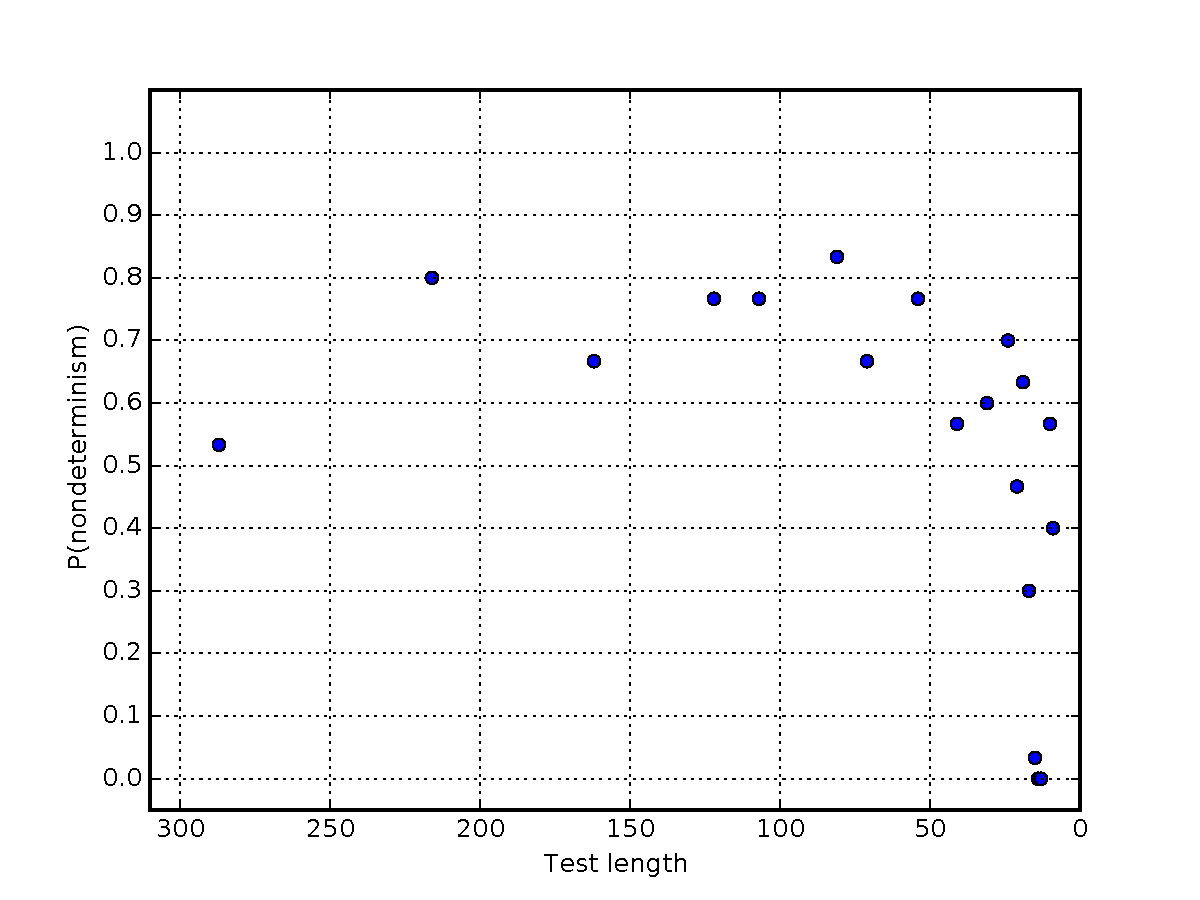
\includegraphics[width=\columnwidth]{redisforcep}
\caption{N=100 (2131s)}
\label{fig:r2}
\end{subfigure}
\begin{subfigure}{0.3\columnwidth}
\centering
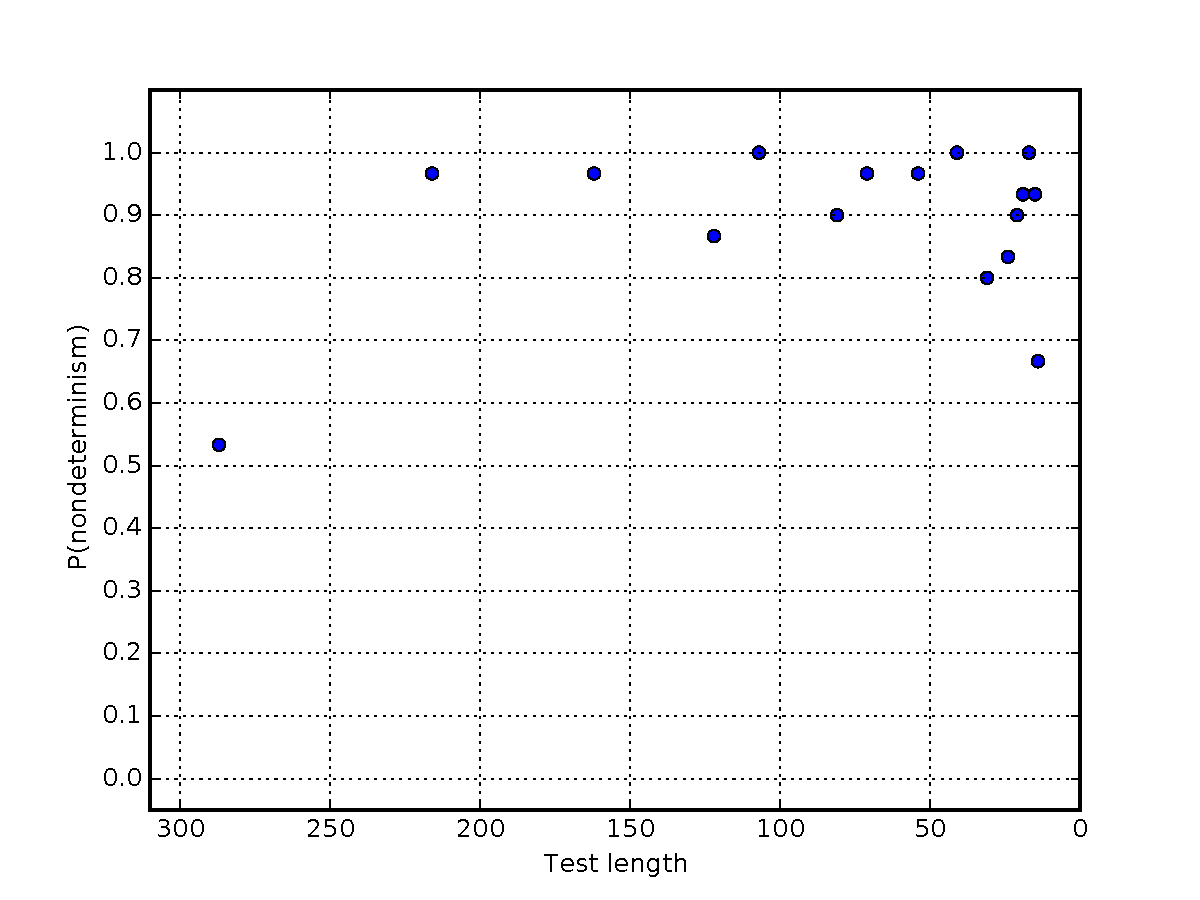
\includegraphics[width=\columnwidth]{redisforceprep}
\caption{M=10, N=10}
\label{fig:r3}
\end{subfigure}
\caption{Reducing a {\tt redis-py} nondeterministic test}
\end{figure}

The {\tt redis-py} \cite{redispy} module implements a (very) widely-used Python interface
to the popular Redis in-memory database, cache, and
message broker \cite{redis}.  
Using TSTL's harness for {\tt redis-py}, both {\tt redis-py} and Redis
itself can be tested; unfortunately, generating stand-alone
high-coverage regression tests for them
has proven difficult, as numerous Redis commands introduce nondeterministic
behavior:  thus the resulting tests are very often \emph{flaky}.
Using AFL, we can see that {\tt redis-py} has a 
stability of only 56.26\%, a clear indicator of significant nondeterminism. Some
of the problematic commands are obvious simply by inspection (e.g.,
{\tt randomkey, srandmember}). It is also clear that 
commands producing data with a limited lifetime (e.g., {\tt expire,
  pexpire}) introduce timing-based nondeterminism.
However, that a command such as {\tt restore} takes an expiration
argument is not obvious to a non-expert, and it is very
difficult to guess whether the {\tt pipe} mechanism, which allows a
large sequence of commands to be queued up and executed
at once, introduces nondeterminism.
\begin{comment}
  Deep experience with Redis would make these
issues clear, but tests using a library are often written by those not
intimately familiar with the semantics of every library call (otherwise they would not have
been as likely to introduce flaky tests in the first place).  This is
even more true in the case of automated test generation, where the
test engineer is often chosen for expertise in test generation tools,
not in the domain of the SUT, and is seldom the
original developer.
\end{comment}

Using the original TSTL harness, just over 20\% of all {\tt redis-py}
regression tests (of length 200) generated were flaky.  Using the
nondeterminism checker to reduce flaky tests to a minimal set allows
us to set up an overnight run that will, in 12 hours, produce
a set of minimal nondeterministic tests exposing the root sources of
nondeterminism/flakiness: we set the harness to repeatedly run, then
produce a regression test.  If the test is flaky (exhibits
nondeterminism in result, over a set of 3 runs), we use the TSTL reducer to shrink it to a
normaliized \cite{onetest} test.  At the end of the testing period,
all distinct tests exhibiting nondeterminism are reported to the
user.  The process reduces the large number of different tests
exhibiting flakiness to a small set of tests, each short, showing a
different cause of nondeterminism.  
There is some duplication of causes, but the tests are sufficient for
identifying all nondeterminism sources.

This process is unlikely to truly require 12
hours, of course; our point is that it is completely automated and
can be given time proportional to the need to find even
low-probability sources of nondeterminism.  The actual amount of time given
may be smaller, or, for that matter, larger (leaving an important
library to self-document nondeterminism over a weekend is hardly a bad
practice).  In this case, the probability of flakiness
is not important, just the possibility, so we let the reducer
create a minimal test with some non-zero (but possibly very small)
observed probability of nondeterminism.  Our 12 hour run identified
all sources of nondeterminism successfully, according to a series of
48 hour runs performed on the version of the harness we modified to
remove nondeterminism, which produced no flaky tests.  We determined that the mean time to find all
the sources of nondeterminism and produce minimal tests is 3.2
hours, which is not trivial, but also, for this purpose, not
excessive.  Our answer to {\bf RQ1} is thus a strong affirmative.

\begin{comment}
\begin{figure*}
{\scriptsize
\begin{code}
{\bf REMOVED:}    
<key> := <r>.randomkey() 
<r>.expire(<key>,<int>)
<r>.pexpire(<key>,<int>)
\{redis.exceptions.ResponseError\} <r>.spop(<key>)
\{redis.exceptions.ResponseError\} <r>.srandmember(<key>)
\{redis.exceptions.ResponseError\} <r>.srandmember(<key>,<int>)
<pipe>.expire(<key>,<int>)
<pipe>.pexpire(<key>,<int>)
\{redis.exceptions.ResponseError\} <pipe>.spop(<key>)
\{redis.exceptions.ResponseError\} <pipe>.srandmember(<key>)
\{redis.exceptions.ResponseError\} <pipe>.srandmember(<key>,<int>)
\vspace{0.1in}
{\bf MODIFIED:}
\{redis.exceptions.ResponseError\} <r>.restore(<key>,<int>,<dump>)
{\bf $\Rightarrow$}
\{redis.exceptions.ResponseError\} <r>.restore(<key>,0,<dump>)
\vspace{0.07in}
\{redis.exceptions.ResponseError\} <pipe>.restore(<key>,<int>,<dump>)
{\bf $\Rightarrow$}
\{redis.exceptions.ResponseError\} <pipe>.restore(<key>,0,<dump>)
\end{code}
}
\caption{{\tt redis-py} calls removed or changed to avoid
  nondeterminism.}
\label{fig:flakysource}
\end{figure*}
\end{comment}

We removed 11 calls from the {\tt redis-py} harness, and  modified 2
calls, after
identification of sources of nondeterminism.  After making these changes, no flakiness was observed in a sample of over 2,000 length
200 tests.   Moreover, because the removals were limited to actually
observed sources of flakiness, the code coverage loss was minimal.
Mean branch coverage, for regression tests of length 200, was reduced
by less than 5 branches (a less than 1\% decrease).  Obviously, it is
impossible to test the removed calls, but the overall coverage loss is
both minimal and known, and can be made up for using specially-crafted
tests (for instance, wrapping the problematic calls in a way that does
not check the values, or adding a delay after an expiration to allow
the data to expire).  As a price to pay for the ability to produce
fast-executing high-coverage full regression tests (not just tests for
crashes and unexpected exceptions), this seems acceptable.  AFL stability was 56.26\% with the harness allowing 
nondeterminism, but rose to 98.32\% using the harness with 
nondeterministic operations removed.

Removing sources of expected nondeterminism also makes
it possible to aggressively test {\tt redis-py} and Redis for
unexpected nondeterminism arising from actual bugs.  The overhead for such
determinism checks, with no delay between operations, is only
20\%, much lower than the expected cost of running each test twice,
answering {\bf RQ2} also in the affirmative.  This is because choosing the actions in a test (and determining which
actions are enabled at each step) consumes a large part of the test
generator's time with a complex library like {\tt redis-py}; running the test again and checking equality is
relatively inexpensive.   

As to {\bf RQ3}, Figures \ref{fig:r1}-\ref{fig:r3} show delta-debugging of a typical
{\tt redis-py} nondeterministic test, originally with 287 steps.  The initial test behaves
nondeterministically about half the time.  Figure \ref{fig:r1} shows
that this is a non-monotonic reduction problem, where removing steps
can either increase or decrease the probability of nondeterminism.  At
first, unmodified delta-debugging actually improves the probability of
failure, but eventually it produces a test of length 16 that only behaves
nondeterministically 24\% of the time.  The reduction takes only 38
seconds.  For the purpose of identifying commands leading to
nondeterminism, this is acceptable.  However, if we were actually
debugging a complex nondeterminism bug in Redis itself, we might want
a more reliably nondeterministic test.  Using the same parameters as
in Section \ref{sec:pubbias}, we see the same pattern.  Simply making
a predicate that ``forces'' the probability to remain high, with a
large number of samples, does not work (Figure \ref{fig:r3}) and
requires over 2,000 seconds to produce a test with an even worse
probability of nondeterminism.  Using 10 samples and 10 replications,
on the other hand, actually improves the probability of
nondeterministic behavior, and (in this case) even produces a smaller test (only 14 steps) in just
over 10 minutes.

\subsubsection{Visible Value vs. Final State Nondeterminism}

We also used {\tt redis-py} to investigate the tradeoff between
overhead and ability to detect nondeterminism when using the two
proposed approaches to horizontal determinism.  We produced 300 tests
of length 100, using the known-nondeterministic version of the {\tt
  redis-py} harness.  We then used {\tt nondeterministic} and {\tt
  stepNondeterministic} calls, both with a delay of 0.005 seconds and
a single additonal execution of the test, to
check these tests for nondeterministic behavior.  Final state
nondeterminism actually detected one instance (but not root cause) of nondeterminism that
visible value nondeterminism failed to detect (21 detections
vs. 20). In general, final state
nondeterminism is less able to detect nondeterminism, but in this
instance the difference is less important than the nondeterminism of
whether a particular test will exhibit nondeterministic behavior in a
single run.  This difference is obviously not statistically
significant; for the nondeterminism in {\tt redis-py}, with these
parameters, the two approaches cannot be statistically distinguished
as to effectiveness in detecting nondeterminism.
Final state nondeterminism was also faster; visible value
nondeterminism took, on average, 0.48\% longer to check for
nondeterminism on the 300 tests, 1.199 mean seconds vs. 1.205 mean seconds.  The difference was significant, with
$p$-value $< 1.19 \times 10^{-23}$ by a paired Wilcoxon test.

\begin{comment}
These results, of course, depend on the parameters of the check for
nondeterminism.  If we increase the delay to 0.01 seconds and the
number of replays of a test used to check for nondeterminism, we
almost double the number of nondeterministic tests discovered.  Both
visible value and final state approaches find 40 nondeterministic
tests, though the overlap of tests thus detected is not quite perfect---each method detects two tests the other does not.  The difference
in overhead, interestingly, is very similar:  0.48\%; however, under
these parameters, visible value nondeterminism is actually cheaper on average
than final state nondeterminism, due to early termination when nondeterminism is detected ($p < 1.44 \times 10^{-10}$).

In practice, we expect that visible value nondeterminism and final state
nondeterminism will often be very similar in both ability to detect
nondeterministic behavior and overhead.  However, under unusual
conditions, the behavior of the approaches can be very different.  The
additional overhead of visible value nondeterminism is usually low
because re-executing a test, not comparing state values for equality, is
the primary cost in nondeterminism detection; however, if there are a
very large number of state components, or some state components have
an expensive equality check (e.g., recursive structures with cycle
detection or depth limits), the overhead can grow, proportional to the
length of tests under consideration.  Similarly, final state
nondeterminism in a setting such as {\tt redis-py}, where divergences
in behavior tend to propagate to other state components, or at least
persist until termination of a test, detects nondeterminism quite
effectively.  However, in a setting where changes in behavior can
easily by overwritten by future test behavior, and do not causally
influence future computation, final state nondeterminism may be almost
useless.
\end{comment}

\subsection{Berkeley {\tt datarray} Inference Algorithms}

\begin{comment}
\begin{figure}[t]
{\scriptsize
\begin{code}
@import inference\_algs
@import datarray
<@
def flat\_sort(v):
    return (sorted(map(flat\_sort,v),key=repr) if type(v) in [list,tuple]
                else (flat\_sort(list(v.items())) if type(v) == dict else v))

def psplit(P):
    return ([P,1.0-P])
@>
pool: <P> 3
pool: <cpts> 3
pool: <evidence> 3 OPAQUE
pool: <ename> 3
pool: <event> 3

<P> := 0.01 * <[0..100]>
<ename> := "E" + str(<[1..5]>)
\{Exception\} <event> := datarray.DataArray(psplit(<P>),axes=[<ename>])
\{Exception\} <ename,1>!=<ename,2> -> <event> := [datarray.DataArray([[
   psplit(<P>)], psplit(<P>)],[<ename>,<ename>])]
<cpts> := []
~<cpts>.append(<event>)
<evidence> := \{\}
~<evidence>.update([(<ename>,0)])

\{Exception\} print(flat\_sort(inference\_algs.calc\_marginals\_simple(<cpts>,
   <evidence>)))
\{Exception\} print(flat\_sort(inference\_algs.calc\_marginals\_sumproduct(<cpts>,
   <evidence>)))
\{Exception\} print(flat\_sort(inference\_algs.calc\_marginals\_jtree(<cpts>,
   <evidence>)))
\end{code}
}
\caption {Complete TSTL harness for finding the hash-order bug in the datarray
  inference algorithms.}
\label{hashbug}
\end{figure}
\end{comment}

The {\tt datarray} module \cite{datarray} is a prototype
implementation for numpy arrays with named axes to improve data
management, developed by the Berkeley Institute for Data Science.  As part of its code, it provides a set of algorithms for
inference in
Bayesian belief networks \cite{russell2016artificial}.  An earlier
version of these algorithms produced nondeterministic (and in some
cases incorrect) results due to dependence on the order of values in
an iterator over a Python dictionary, on Python versions above 3.2,
until 3.6 (see Section \ref{sec:pnondet}).  

\begin{comment}
Figure \ref{hashbug} shows TSTL code for generating inputs to the {\tt
  datarray} algorithms.  The {\tt flat\_sort} function is
needed because we care about actual differences in probability values,
not simply the order of list, tuple, or dictionary items.
\end{comment}
Running our TSTL
harness to test {\tt datarray} consistently requires less than 10 seconds to produce a test exhibiting process-level nondeterminism in
the {\tt calc\_marginals\_sumproduct} function (the only broken
algorithm), answering {\bf RQ1} again in the affirmative.  Reducing this 60 step test to a minimal test of only 6 steps,
showing an extremely simple input producing the issue, 
required another 92 seconds ({\bf RQ3}) on average.  Interestingly, the way that {\tt
  python-afl} is used in TSTL means that AFL stability is 100\% even
for the original, broken, code,
because the {\tt PYTHONHASHSEED} has already been chosen before the
fork in AFL.  Removing the nondeterministic call, we can see that the cost of
checking for process nondeterminism, with no delay between operations,
is high, a mean 93\% slowdown ({\bf RQ2}.  This is due to the high cost of subprocess
creation and communication. However, even with this essentially worst
case behavior (where test runtime is very low compared to process overheads),
we don't quite halve test executions.

\subsection {Vertical Determinism: {\tt pyfakefs}}

The {\tt pyfakefs} \cite{pyfakefs} module implements a fake file
system that mocks the Python file system modules, to allow Python
tests both to run faster by using an in-memory file system and to make
file system changes that would not be safe or easily performed using
real persistent storage.  Originally developed in 2006 at Google by
Mike Bland, {\tt pyfakefs} is now used in over 2,000 Python tests,
inside and outside Google \cite{pyfakefs}.
The TSTL harness for {\tt pyfakefs} has been used to detect (and
correct) over 80 faults.
%\url{https://github.com/jmcgeheeiv/pyfakefs/issues?q=label\%3ATSTL}.  

\subsubsection{Manually Inserted Fault}

We introduced a subtle bug into {\tt pyfakefs}, where the {\tt remove}
call checks that its target is not a directory, and returns the
correct error, but still carries out the remove.  Using {\tt
  os.remove} to delete directories violates the Python {\tt os}
specification (and the POSIX standard).  Detecting this bug using the TSTL
{\tt pyfakefs} harness is normally impossible without using another
file system as a reference.  However, the fault was detected  essentially
immediately with our failure determinism checks (an affirmative answer
to {\bf RQ1}).  Moreover, the overhead for the check in a
version of the code without the error was
less than 8\%  ({\bf RQ2}).  Detecting the fault using a reference file system 
required 17\% more testing time before detection, and took over twice as
long to reduce the failure, to a
slightly longer failing test, which did not have {\tt remove} as its
final operation (since further operations are required to 
expose the bad state).
Because vertical
reduction does not require running complete tests multiple times, and
does not affect the delta-debugging algorithm's performance, reducing
the failing test to 3 steps required less than a second ({\bf RQ3}).
Here, failure determinism even improves on hand-tuned differential testing.

\subsubsection{Mutation Analysis}

We wanted to determine whether there were also simple faults that
could be detected by failure nondeterminism, but \emph{not} detected
by differential testing, and quantify the additional specification
strength provided by failure determinism checks, to further answer
{\bf RQ1} in the special case of failure determinism.  We therefore used
{\tt universalmutator} \cite{RegExpMut} to produce 2,350 mutants of
the {\tt pyfakefs} core file system code.   %We restricted the generation
%to only mutate code covered during a 60 second run of the test
%harness.
\begin{comment}
  We could have applied mutation
testing to {\tt redis-py}, but we are dubious of the value of such an
analysis without a strong differential harness to compare to; the {\tt
  redis-py} testing is limited in strength, and largely useful for
producing high-coverage operation sequences from which to construct
manual unit tests.


In each run we first analyzed the mutants using 60 seconds of non-differential
testing \emph{without failure nondeterminism checks}, then with the
full differential harness (also without failure nondeterminism checks)
for 120 seconds; the additional 60 seconds is to make sure we accounted for the observed 17\%
extra time to detect in the manually constructed example: we want to
maximize the chance to detect a bug using the strong version of the harness.   For both comparisons, we then tested
all surviving mutants using a non-differential harness for 60
seconds, this time with failure nondeterminism checking.
%We used the same random seed for
%all runs, so that the only differences would be specification-based.
\end{comment}

Non-differential testing, without failure determinism checks,
consistently (in all runs) killed
872 mutants, a 37.1\% kill rate.
%Adding a failure determinism check
%allowed the testing to (again, consistently) kill an additional 98 mutants, an 11\% improvement.
The differential harness, with an additional 60 seconds of testing
time (to make sure we accounted for the observed 17\%
extra time to detect in the manually constructed example: we want to
maximize the chance to detect a bug using the strong version of the harness), consistently killed 1,148 mutants, improving the kill rate to 48.8\%.  Failure
nondeterminism checking consistently added an
additional 71 mutants to that total, \emph{a 6\% improvement even for
this strong differential harness with a larger test budget}, nearly as
large an improvement as the gain from using a full reference
implementation for comparison.  Using
failure nondeterminism was the \emph{only} way to push the mutation score
above 50\%.  The kill rates are generally low
because {\tt universalmutator} includes many operations
thatproduce hard-to-kill
non-equivalent mutants not produced by other mutation tools.  This is a strong affirmative answer to {\bf
  RQ1}.

\begin{comment}
In order to further investigate the additional specification power
provided by failure nondeterminism detection, we inspected the mutants
killed using the failure determinism check but not killed by the
strong differential testing.  The largest category of mutants not
killed (22 of the 71 mutants) was what we refer to as ``exception
swallowing'' mutants, which transform a Python statement into the same
statement, but wrapped in a {\tt try} block with a catch that ignores
any raised exceptions.
It is easy to
see that such mutants may introduce faults in the handling of
errors, and thus would tend to cause failure nondeterminism.  Other mutation operators resulting in subtle flaws
not (at least easily) detectable by differential testing compared to a
correct file system included:  arithmetic operation changes, statement
deletions, logical operator modifications, constant replacements
(including replacement of a string with the empty string), and
introducing a break into a loop.  The variety of mutant types suggests
that no more specifically tailored strategy such as checking for
exception propagation, will work as well as introducing a notion of
failure nondeterminism.  This is a strong affirmative answer to {\bf
  RQ1} at least for a large set of hypothetical bugs.

We also checked the cost of introducing failure determinism checking
by analyzing mutants that could be killed by both methods ({\bf RQ2}).  Even
though in some cases the failure determinism check allows a mutant to
be detected sooner, the mean time to kill mutants was 0.006 seconds
larger with failure determinism checking, and this change was significant by Wilcoxon test
$(p < 1 \times 10^{-15})$.  While \emph{statistically} significant,
this cost is almost certainly
too small to be of any real practical importance.
\end{comment}


\begin{comment}
\subsection{Summary of Results}

\begin{itemize}
\item {\bf RQ1: Is our approach able to reliably detect
  nondeterminism?}  For all of our subjects, all nondeterminism we are
aware of was detected.  The {\tt pyfakefs} experiments also show,
using mutation testing, an additional ability to detect bugs over a
strong differential test.
\item {\bf RQ2: Is the overhead of nondeterminims detection
    acceptable?} This depends on the criteria for acceptability, but
  given the fault-detection and flaky-test avoidance capabilities
  demonstrated, we think that so long as the testing is still able to
  execute at least half as many tests, for the same time budget, the
  answer is yes.  All subjects, even when using expensive
  process-based checks, satisfied this constraint.  Failure
  nondeterminism detection was particularly inexpensive, as expected.
\item {\bf RQ3: Is the performance of delta-debugging/test reduction
    acceptable?}  In all cases, reduction was relatively quick (a
  little over 10 minutes in the worst case) and the amount of
  reduction produced was large (85\% or better).
\end{itemize}
\end{comment}

\subsection{Threats to Validity}

There are several primary threats to validity:  first, our empirical
results are limited to a small set of Python programs, ranging from
relatively small and simple to large and complex libraries; the
representative nature of these subjects is not clear.
Because
no other tools implement the kind of approach taken here, we were unable
to perform a meaningful comparison with another nondeterminism
detection tool.  DeFlaker \cite{bell2018d}
performs a completely different task, and cannot check
nondeterminism at any smaller granularity than a whole test.  iDFlakies
\cite{idflakies}, similarly, ``does not further classify the causes of
the flaky tests'' beyond identifying them as likely related to test
order.  
Another threat to validity is posed by implementation errors.
%TSTL and the mutation tool are tested for bugs by a set of Travis CI
%tests, and the nondeterminism
%detected by TSTL can be demonstrated with standalone tests.
\section{Related Work}

At a very broad level, the topic of uncertainty (and thus nondeterminism) in software engineering has been addressed by Garlan \cite{GarlanUncertain}, Elbaum and Rosenblum \cite{Unknowns,lu2015roundtable}, and Ziv and Richardson \cite{UncertaintyPrinciple}.  There is a general agreement that as systems become more complex, more distributed, and more \emph{statistical}, these problems will only grow \cite{lu2015roundtable}.

Gao et al. generally considered the question of how to make tests repeatable \cite{Gao:2015:MSU:2818754.2818764}, in the context of system-wide user interaction tests.  Their work focused on systemic factors, such as execution platform and persistent configuration and database files, in contrast to our focus on identifying nondeterminism at the library level.  However, what they refer to as ``test harness factors'' includes delays, which can be of importance to nondeterminism at the library level when asynchronous behavior is involved.

Shi et. al \cite{DetermImp} examined what might be seen as a related, though in a sense the opposite, problem:  they detect code that assumes a deterministic implementation of a non-deterministic specification.  E.g., they detect instances when  iteration through items of a set is explicitly not guaranteed to provide any particular order of items, but code depends on the order produced by a given implementation.  This procedure, applied to Python code in a pre-3.3 environment, would have flagged many instances of the nondeterminism that arose on the introduction of salted hashing.  Determinism is also sometimes used as a property in domain-specific testing efforts, e.g. in testing shader compilers \cite{shader}.

The problem of test nondeterminism is closely related to the (extremely important in industrial settings) issue of flaky tests \cite{miccoflaky, luo2014empirical,palomba2017does,listfieldtestanalysis}.  How to handle flaky tests in practice (when they cannot be avoided) is a major issue in Google-scale continuous testing \cite{memon2017taming}, and, as Memon et al. describe, the problem of flaky tests influences the general design of Google test automation.
Previous work on flaky tests has either focused on test inter-dependence as a cause of flaky behavior \cite{LamZE2015}, or provided large-scale empirical examination of tests from one large open source project (Apache) \cite{luo2014empirical,palomba2017does}.  Palomba and Zaidman \cite{palomba2017does} investigated the relationship between test code smells and flaky tests.   The present paper, rather than focusing on flaky tests per se, investigates new tools for handling nondeterminism in property-based test generation.  From our point of view, flaky behavior is simply a special case of nondeterminism, where the nondeterminism is sufficient to cause the test to have different pass/fail results at times.  Our approach is, in a sense (especially the delta-debugging modifications) in line with Harman and O'Hearn's proposal to simply accept that ``All Tests Are Flaky'' \cite{StartupstoScaleups}, and work with probabilistically failing tests.

Other efforts \cite{ParallelDeterministic} have aimed to avoid nondeterminism in parallel implementations, by design, indicating the importance of avoiding nondeterministic behavior, even at the expense of adopting novel programming models, where the goal is not simply (as in, say, Rust) to avoid classic concurrency errors, but to enforce genuinely deterministic behavior.  

Finally, Cotroneo et al. \cite{CompBugs,FaultTriggers}, and Grottke and Trivedi \cite{GrottkeBugs} have followed on early work on understanding bugs and how they manifest, including transient \cite{Transient} software faults.  This work informs our attempt to identify sources of nondeterminism, and should provide other, context and project-specific, sources that could be introduced into our general framework.



\section{Conclusions and Future Work}

Unexpected nondeterminism of software systems frustrates users,
whether they be humans or (more importantly) other software systems.
Nondeterminism is even more pernicious in software testing,
frustrating debugging efforts (Heisenbugs \cite{Heisenbug} and
Mandelbugs \cite{GrottkeBugs,FaultTriggers} are widely loathed), and
leading to the costly problem of flaky tests
\cite{miccoflaky,listfieldtestanalysis}.
This paper proposes a formulation of types of nondeterminism, and a
practical approach to using automated test generation to detect and understand
nondeterminism, especially in the library code that underlies most
systems. In addition to traditional \emph{horizontal} nondeterminism, we introduce
the concept of \emph{vertical} nondeterminism bugs, and show their
additional specification power compared to a
strong differential testing harness.  
\begin{comment}
We implemented our approach in the
TSTL automated test generation system for Python, and demonstrated the
simplicity and utility of the approach on real-world examples.


As future work, we would like to support the automatic detection of opaque
values; if a value (e.g., a timestamp) is different in \emph{every}
trace, it is likely opaque.  This would make
testing libraries with intended nondeterminism much easier. Similarly, for
vertical nondeterminism, we would like to
automatically identify idempotent operations.
%We would also like to lower the cost
%of checking process nondeterminism, perhaps by using methods taken in
%AFL \cite{aflfuzz} to avoid high startup costs for test executions.
Finally, we are interested in using test decomposition
\cite{Composition} to isolate and understand
nondeterminism in unit tests, and to mitigate flaky tests.
Reliable detection of nondeterminism is a critical tool in making such
an approach efficient and reliable.
\end{comment}

\begin{comment}
Finally, it would be useful to implement versions of our formalisms in
test generation tools for other languages with a suitable notion of
action.  For example, the DeepState
\cite{DeepState,DeepStateTutorial,deepstaterepo} tool for
property-based fuzzing and symbolic-execution of C and C++ code defines
actions that are choices between C++ lambdas in a test harness,
produced by a nondeterminism operator, {\tt OneOf}.
Adding annotations of visible state (perhaps simply in the form of
blocks of address ranges in memory, a method often suitable for C and
C++ code) would make it possible to search for unexpected nondeterminism in
critical C and C++ libraries.

{\scriptsize {\bf Acknowledgments:}  The authors would like to thank John Micco,
Jeff Listfield, and Celal Ziftci at Google, for discussion of
flaky tests, Andreas Zeller and David R. MacIver for discussion of the
problem of probabilistic delta-debugging, and Chris
Colohan for discussion of sources of process-based nondeterminism.}
\end{comment}


\bibliographystyle{plain}
\bibliography{bibliography}

\end{document}
